\chapter{Klassen und Objekte}

\section{Lösungsvorschlag}


\begin{minted}[mathescape,
    linenos,
    numbersep=5pt,
    gobble=2]{java}
    public class Omnibus extends Auto {
        private int anzahlSitzplaetze;
        public Omnibus(
                int anzahlSitzplaetze,
                int kmStand,
                double verbrauch,
                double tankVolumen,
                double kraftstoffVorrat) {
            super(kmStand, verbrauch, tankVolumen, kraftstoffVorrat);
            if (anzahlSitzplaetze > 0) {
                this.anzahlSitzplaetze = anzahlSitzplaetze;
            }
        }

        public String toString() {
            return "anzahlSitzplaetze: " + anzahlSitzplaetze +
                    "; " + super.toString();
        }
    }
\end{minted}\\

\section{Anmerkung und Ergänzungen}

\begin{itemize}
    \item \code{Omnibus} ist eine \textit{Spezialisierung} von \code{Auto}, umgekehrt ist
    \code{Auto} eine \textit{Generalisierung} von \code{Omnibus} (s. Abbildung \ref{fig:omniuml})
    \item Der Konstruktor wird um einen formalen Parameter \code{anzahlSitzplaetze} erweitert.
    \item Ein \code{Omnibus} ist ein \code{Auto}\footnote{\textit{Fahrzeug} würde als Generalisierung vlt. etwas besser passen} und verhält sich auch so: Es kann alles tun, was ein \code{Auto} tun kann, und deshalb können alle Methoden auch in \code{Omnibus} wiederverwendet werden.
    \item Die Vererbung schließt nicht die in \code{Auto} als \code{private} deklarierten Attribute mit ein - diese stehen der Klasse \code{Omnibus} nicht zur Verfügung.
    Ein Zugriff auf als \code{private} deklarierte Felder über Methoden, die \textbf{public}, \textbf{protected} oder \textbf{package-private}\footnote{\textit{package access}, s. \url{https://docs.oracle.com/javase/specs/jls/se21/html/jls-6.html#d5e11105} - abgerufen 8.2.2024} sind, ist aber trotzdem möglich\footnote{s.a. ``Private Members in a Superclass``: \url{https://docs.oracle.com/javase/tutorial/java/IandI/subclasses.html} - abgerufen 8.2.2024}.\\
    Gleiches gilt für den Konstruktor, der die Initialisierung der Felder \code{kmStand}, \code{verbrauch}, \code{tankVolumen}, \code{kraftstoffVorrat} übernimmt.
    \item Der erste Aufruf in einem Konstruktor muss stets den Konstruktor der Elternklasse aufrufen.\\
    Fehlt solch ein expliziter Aufruf, erfolgt ein \textit{impliziter} Aufruf durch den Compiler.\\
    Soll \textit{explizit} der Konstruktor der Oberklasse aufgerufen werden, muss dieser Aufruf als erstes erfolgen.\\
    Erst danach darf das Attribut \code{anzahlSitzplaetze} initialisiert werden\footnote{
    Nachdem Aufrufe zu \textit{this()} bzw. \code{super()} erfolgt sind und die Initialisierung der Attribute des zu erzeugenden Objektes abgeschlossen sind, wird die übrige Konstruktorimplementierung abgearbeitet. S.a. ``12.5 Creation of New Class Instances``: \url{https://docs.oracle.com/javase/specs/jls/se21/html/jls-12.html#jls-12.5} - abgerufen 8.2.2024
    }.
    \item Eine sinnvolle Initialisierung von \code{anzahlSitzplaetze} erfolgt mit Werten $> 0$.
    (standardmäßig erfolgt die Initialisierung von Objekt-Attributen vom Typ \code{int} mit dem Wert $0$ (vgl.~\cite[127]{Ull23})).
\end{itemize}


\begin{figure}
    \begin{center}
    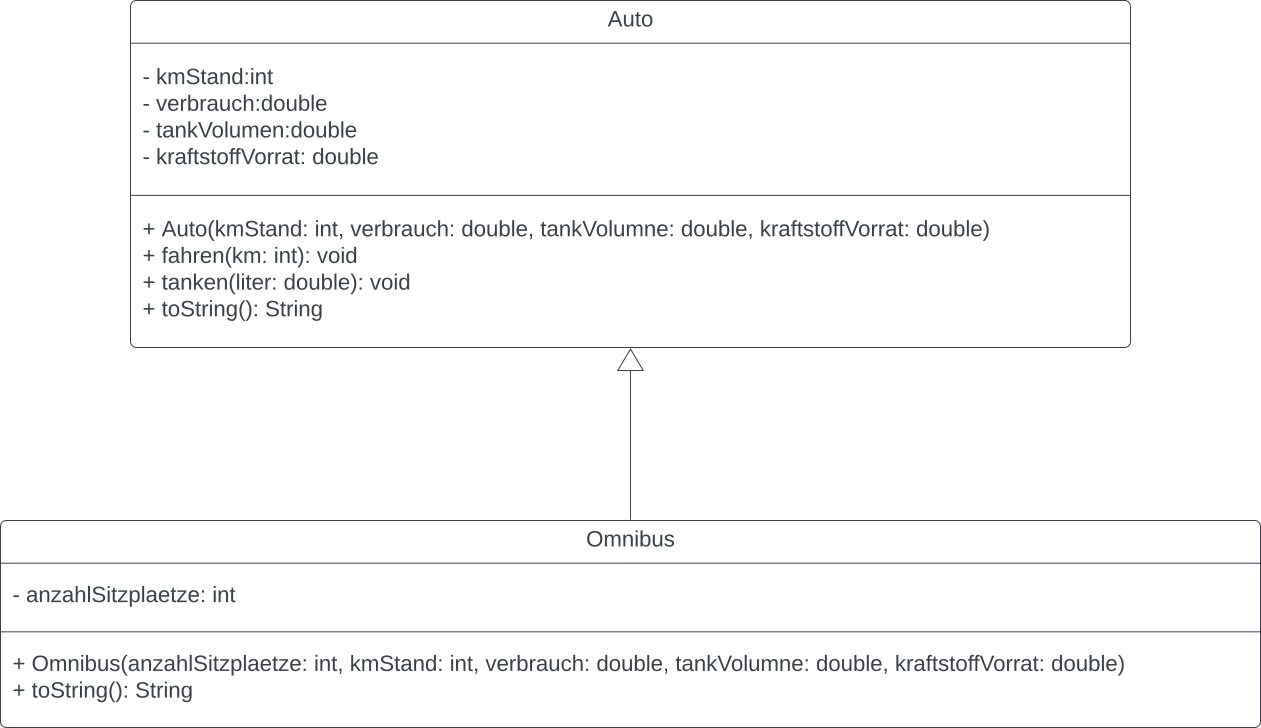
\includegraphics[scale=0.3]{chapters/2. Vererbung/img/omniuml}
    \caption{Das UML-Klassendiagramm für die Generalisierungsbeziehung zwischen \textit{Omnibus} und \textit{Auto}}
    \label{fig:omniuml}
    \end{center}
\end{figure}
